\documentclass[../mciAusarbeitung.tex]{subfiles}

\usepackage[utf8]{inputenc}
\usepackage[T1]{fontenc}
\usepackage{lmodern}
\usepackage[german]{babel}
\usepackage[fixlanguage]{babelbib}
\selectbiblanguage{german}
\usepackage{amssymb}
\usepackage{graphicx}
\usepackage{url}
\usepackage{float}
\usepackage{wrapfig}

\title{Fachpraktikum MCI (01513) - WS 2021/22}
\author{Gruppe 2\\
	Bastian Winzen}
\date{\today}

\begin{document}
Im Folgenden werden drei im Fachpraktikum entwickelte Implementationen von Bildgeneratoren vorgestellt. Die Ausarbeitungen basieren auf einem Algorithmus zur Schwarm Simulation, der Berechnung und Darstellung von Lindenmayer-Systemen (L-Systeme) oder befolgen Evolutionsprinzipien zur Erstellung eines Bildes.


\subsubsection{BWinzen::Schwarm - Schwarm Simulation}
	Die Entwicklung einer Schwarm Simulation erfolgte nach dem Vorbild der Flocking Simulation von Craig W. Reynolds aus dem Jahre 1986 \cite{reynolds1987flocks}.
	Kern dieses Ansatzes ist es, dass jedes Element im Schwarm sich selbst organisieren und ausrichten kann. Jedes dieser Elemente kennt seine Position, seine aktuelle Geschwindigkeit und kann auch diese Werte von allen anderen Elementen im Schwarm erfassen. Reynolds bezeichnet diese Elemente als ``Boids'', eine Wortneuschöpfung aus Bird und Android, die eine künstliche Simulation von Vogelverhalten andeutet.\\
	
	Um als ein Schwarm wahrgenommen zu werden müssen viele einzelne Komponenten in der Wahrnehmung zu einer Einheit bzw. Gruppe verschmelzen. Folgende Kriterien unterstützen diese Einordung: 1. \textit{Prinzipien der Wahrnehmung}: Gruppierung durch Form und Größe/Minimierung des Popup Effektes. Die Elemente weisen eine ähnliche Form und Größe auf. 2. \textit {Phänomene der Wahrnehmung}: ``gemeinsames Schicksal''. Geringe Entfernung, gleiche Geschwindigkeit und Ausrichtung implizieren eine Einheit. \cite{PetersSS21EMCI}.\\
	
	Um das Verhalten eines Schwarms zu simulieren, werden von Reynolds drei Grundkräfte genannt, die auf die Boids einwirken. Diese errechnen sich individuell für alle Elemente aus den Positionen und Geschwindigkeiten aller anderen Elemente im Schwarm.
	\begin{itemize}
	\item[]Die erste genannte Kraft ist die \textbf{``Collision Avoidance''} - zu Deutsch \textbf{Separationskraft}. Diese soll eine Kollision zwischen zwei Boids verhindern. Je näher sich zwei Elemente sind, desto stärker wird ihr Bestreben sich von einander zu entfernen.
	\item[]Die zweite genannte Kraft ist das \textbf{``Velocity Matching''} - zu Deutsch \textbf{Ausrichtungskraft}. Diese soll Boids so ausrichten, dass sich ihre Bewegungsvektoren immer mehr angleichen.  
	\item[]Die dritte genannte Kraft ist das \textbf{``Flock Centering''} - zu Deutsch \textbf{Kohäsionskraft}. Sie ist die Gegenkraft zur Separation und verhindernd ein zu starkes Auseinanderdriften der Boids. Der Kraftvektor zeigt auf den errechneten Mittelpunkt aller Elemente und bezeichnet die Intention aller Elemente sich an einem einzelnen Punkt im System zu versammeln.
	\end{itemize}
	
	Je nach Zusammenspiel dieser 3 Kräfte ergibt sich ein unterschiedliches Bild. Für die Implementation im Rahmen dieses Praktikums wird jede Kraft vom Anwender mit einem Faktor konfiguriert. So kann der Nutzer bestimmen ob er gleichmäßig verteilte Boids oder Boids, die sich in wenigen Punkten sammeln sehen möchte.\\
	In welchem Radius die Boids für die Berechnung der drei Grundkräfte herangezogen werden ist einzeln für jede Kraft konfigurierbar.\\\\
	Das berechnen der Kräfte für jedes Element im Schwarm hat eine Laufzeit von $O(n^2)$ wobei n der Anzahl aller Elementen entspricht. Für die Berechnung eines Elements muss immer jedes andere Element herangezogen werden.
	Die Konfiguration des Radius schränkt die Auswahl der Elemente, welche in die Berechnung der Kräfte einfließen jedoch ein. Um die Elemente im Radius zu ermitteln müssen dennoch zunächst alle Boids betrachtet werden.
\begin{wrapfigure}{r}{0.5\linewidth}
	\center
	\includegraphics[width=8cm]{"img/quadtree.png"}
	\caption{Beispiel eines Quadtrees entnommen aus \cite{DavidEppstein2005}}  
\end{wrapfigure}	
	Dieses Laufzeitverhalten stellt ein Problem dar, wenn die Anwendung auch mit vielen Boids flüssig laufen soll. \\
	Um meine hohe Anzahl Boids in der Anwendung zu ermöglichen wurde ein Quadtree implementiert und für die Datenhaltung der Boids verwendet. Dieser ermöglicht das Prinzip ``Divide and Conquer'' im zweidimensionalen Raum. Zusammengefasst kann der der Quadtree wie folgt beschrieben werden: \\
	Jedes Baumverzeichnis hat feste geometrische Grenzen. Zudem kann jedes Baumverzeichnis nur eine maximale Anzahl an Objekten beinhalten. Wird die maximale Anzahl überschritten wird der Bereich in 4 Teilbereiche unterteilt für die jeweils ein Baumverzeichnis instanziiert wird. Die Objekte werden nach ihrer räumlichen Anordnung in die entsprechenden Unterverzeichnisse einsortiert.\\	
	Durch die Nutzung des Quadtrees können Elemente mit einer Laufzeit von Durchschnittlich $O(ln(n))$ anhand ihrer Position gefunden werden bzw. alle Elemente in einem Radius gequeryt werden. Die Laufzeit pro Iteration beläuft sich auf $O(n*ln(n))$ \cite{Samet}.\\
	Um die Performance des Schwarms zu verbessern wurde die Berechnung vom Zeichenvorgang abgekoppelt. Boids haben 2 Zustände, den aktuellen Zustand sowie den Zustand für die nächste Iteration. In jeder Iteration wird der neue Zustand errechnet. Dies geschieht multithreaded und zur Berechnung werden die aktuellen Status der anderen Boids verwendet. Sind alle neuen Zustände berechnet werden sie als aktuell gesetzt und die Boids werden gezeichnet. Da die Renderer Statemachines sind, muss das Zeichnen synchron ablaufen.\\
	Bei den Schnittstellendefinitionen der Boids wurde darauf geachtet, dass zusätzlich zu den drei Grundkräften eine weitere Kraft in die Berechnung des neuen Zustands einfließen kann. Ein Beispiel für eine solche Kraft ist die Anziehung oder Abstoßung eines im Kooperation Kontext definierten Punktes.\\
	Ein weiteres Feature der Implementierung ist die Farbdiffusion. Mit entsprechenden Einstellungen wird die Farbe der Boids in jeder Iteration neu berechnet. Dafür werden die Farben der Boids im kleinsten der gewählten Radius zusammengerechnet und ein Durchschnittswert errechnet. Dieser Farbwert wird als neuer Farbwert des Boids gesetzt. Zudem gibt es eine spezielle Möglichkeit der Kooperation, bei der die Boids die Farbe des Pixels der aktuellen Position aus der vorangegangenen Iteration übernehmen. Dafür muss in den Parametern ein entsprechender Filter definiert werden, der definiert welche Farbwerte übernommen werden.
	
\paragraph{Parameter-Beschreibungen für BWinzen::Schwarm}
\begin{itemize}
	\setlength\itemsep{-0.1em}
	\item\textit{Anzahl:} Anzahl der Boids in der Simulation
	\item\textit{Ausrichtung:} Faktor für die Gewichtung der Ausrichtung
	\item\textit{Kohäsion:} Faktor für die Gewichtung der Kohäsion 
	\item\textit{Separation:} Faktor für die Gewichtung der Separation 
	\item\textit{Radius Aus.:} Radius für die Betrachtung anderer Boids zur Berechnung der Ausrichtung
	\item\textit{Radius Sep.:} Radius für die Betrachtung anderer Boids zur Berechnung der Separation
	\item\textit{Radius Kohäsion:} Radius für die Betrachtung anderer Boids zur Berechnung der Kohäsion
	\item\textit{Form:} Form der Boids. Derzeitige Varianten: {Kreise, Linien, Pole, Rechtecke, Quadrate, Dreiecke, Zufällige Formen}
	\item\textit{Größe:} Größe der Boids
	\item\textit{Feste Größe:} Aktiviert - Alle Elemente die gewählte Größe, Deaktiviert - Größe zufällig und maximal Wert begrenzt
	\item\textit{Anfangsfarbe:} Grundlage zur Berechnung der Elementfarbe 
	\item\textit{Farbmodus:} siehe \ref{parametrisierung} Allgemeine Parametrisierung>>Farbmodus
	\item\textit{Farbverläufe:} Aktiviert -  Alle Boids aus dem kleinsten Radius der drei gewählten Radius werden zur Berechnung der nächsten Farbe herangezogen. Für jeden Farbkanal wird der Durchschnittswert aller Boids im Radius errechnet und als neue Farbe gesetzt.
	\item\textit{CoopModus Farbenübernahme:} Das aktuelle Pixel des bestehenden Bildes wird pro Iteration über Filter geprüft. Wenn der bestehende Farbwert dem ausgewählten Filter genügt, wird der Farbwert übernommen. Aktuelle stehen folgende Filter zur Verfügung:
		\begin{itemize}
		\setlength\itemsep{-0.1em}
			\item Keine Übernahme,
			\item Hohe Farbkanal Werte (> 0xF8),
			\item Mittel Starke Farbkanal Werte (> 0xC4),
			\item Schwache Farbkanal Werte (> 0x80),
			\item Starker Rot Wert (> 0xF8),
			\item Starker Grün Wert (> 0xF8),
			\item Starker Blau Wert (> 0xF8),
			\item Starker Blau Wert (> 0xF8), Helle (Brightness > 0.7),
			\item Dunkle (Brightness < 0.3),
			\item Hohe Sättigung (Saturation > 0.7)
		\end{itemize}
	\item\textit{KoopModus Orientierung:}  siehe \ref{parametrisierung} Allgemeine Parametrisierung>>KoopModus Orientierung
	\item\textit{Max. Geschwindigkeit:} Maximale Geschwindigkeit der Boids.
	\item\textit{Max. Beschleunigung:} Maximale Beschleunigung der Boids. Je höher der Wert, desto abrupter sind die Richtungswechsel.
	\item\textit{Einheitliche Geschwindigkeit:} Aktiviert - Alle Boids die gleiche Geschwindigkeit. Diese Option hat sehr großes Einfluss auf das Verhalten des Schwarms.
	\item\textit{Kanten Verhalten:}
		\begin{itemize}
		\setlength\itemsep{-0.1em}
			\item\textit{Konzentrisch:} Verlassen die Boids das Fenster, werden sie auf die Gegenseite versetzt. Dabei wird die Richtung beibehalten.
			\item\textit{Spiegeln:} Verlassen die Boids das Fenster, wird ihr Geschwindigkeitsvektor an der Kante die überschritten wurde, gespiegelt.
			\item\textit{Rotation:} Sind die Boids dabei das Fenster zu verlassen, werden sie abgeleitet/rotiert bis sie wieder in Richtung des Fensters fliegen. Je schneller sie fliegen um so stärker ist die Rotation ausgeprägt.
			\item\textit{Teleportation:} Verlassen die Boids das Fenster, werden sie an den Punkt des Kooperationskontextes teleportiert behalten aber ihren Richtungsvektor. Wenn die überschrittene Kante zu nah am Zielpunkt liegt wird der Richtungsvektor umgedreht.
		\end{itemize}	
	\item\textit{Farbenreservoirs nicht zeichnen:} Um Farben zur Übernahme in der Cooperation zu haben, wurden zu Testzwecken `Farbenreservoirs' gezeichnet. Zufällig wird ihre Farbe gesetzt und dabei darauf geachtet, dass die Farben übernommen werden können. Die `Farbenreservoirs'  sind Kreise die mit Gradienten gefüllt sind. Ihre Farbe und Bewegung wird durch den Seed zufällig bestimmt. Implementiert ist ein Rotation sowie ein alternierendes auseinanderdriften der Kreise. Diese beiden Eigenschaften können kombiniert werden, wodurch ein Spiralverlauf entsteht.
	\item\textit{Farben verblassen:} Diese Einstellung kommt nur zum Tragen wenn der Verlauf eingeschaltet ist. In jeder Iteration werden alle Pixel des Layers in ihrer Opacity um den eingestellten Wert verringert.
\end{itemize}	
%\pagebreak
\paragraph{Beispiele:}
Folgende Beispiele können im Konfigurator unter MenuBar>>Beispiele>>BWinzen>>Schwarm ausgewählt werden.

	\subparagraph{a)Batcave:} Dreiecke in einem Schwarm, die ihre Farbe an den Nachbarn anpassen und beim Überflug über Bildpunkte mit starken Farbkanalwerten (r oder g oder b über 0xF8) die Farbe des unterliegenden Pixels annehmen.	
	
	\subparagraph{b)2 Schwärme:} 2 Schwärme mit unterschiedlichem Randverhalten, Größe, Form und anderen Parametern.

	\subparagraph{c)Colorexplosion:} Ein Schwarm bestehend aus Linien. Die aktuelle wird mit der vorherigen Position des Boids durch eine Linie verbunden. Der Verlauf ist eingeschaltet und es wird in jeder Iteration der Alpha Wert des bestehenden Verlaufs um 10 reduziert.

	\begin{figure}[H]
		\begin{subfigure}{0.5\linewidth}
			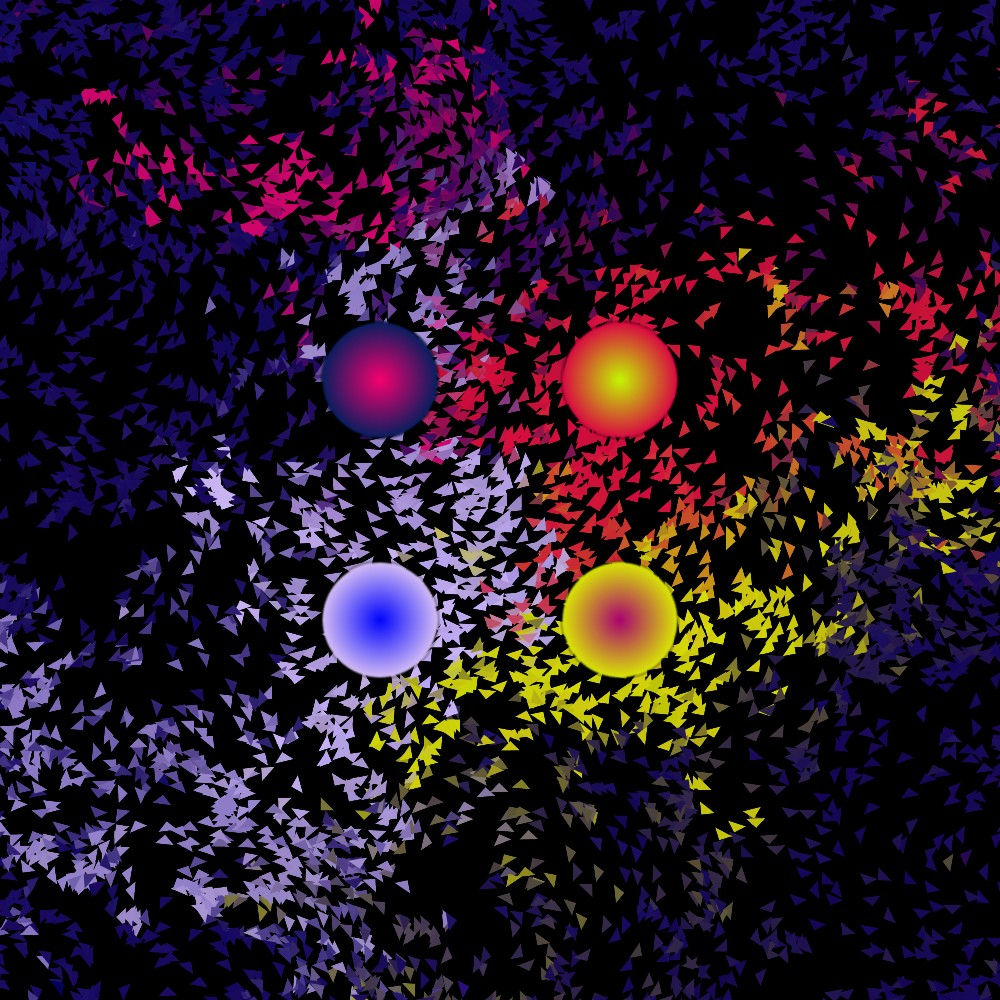
\includegraphics[width=0.95\linewidth]{"img/swarm_batcave.jpg"}
			\caption[Batcave]{\textbf{Batcave}}  
		\end{subfigure}	
		\begin{subfigure}{0.5\linewidth}
			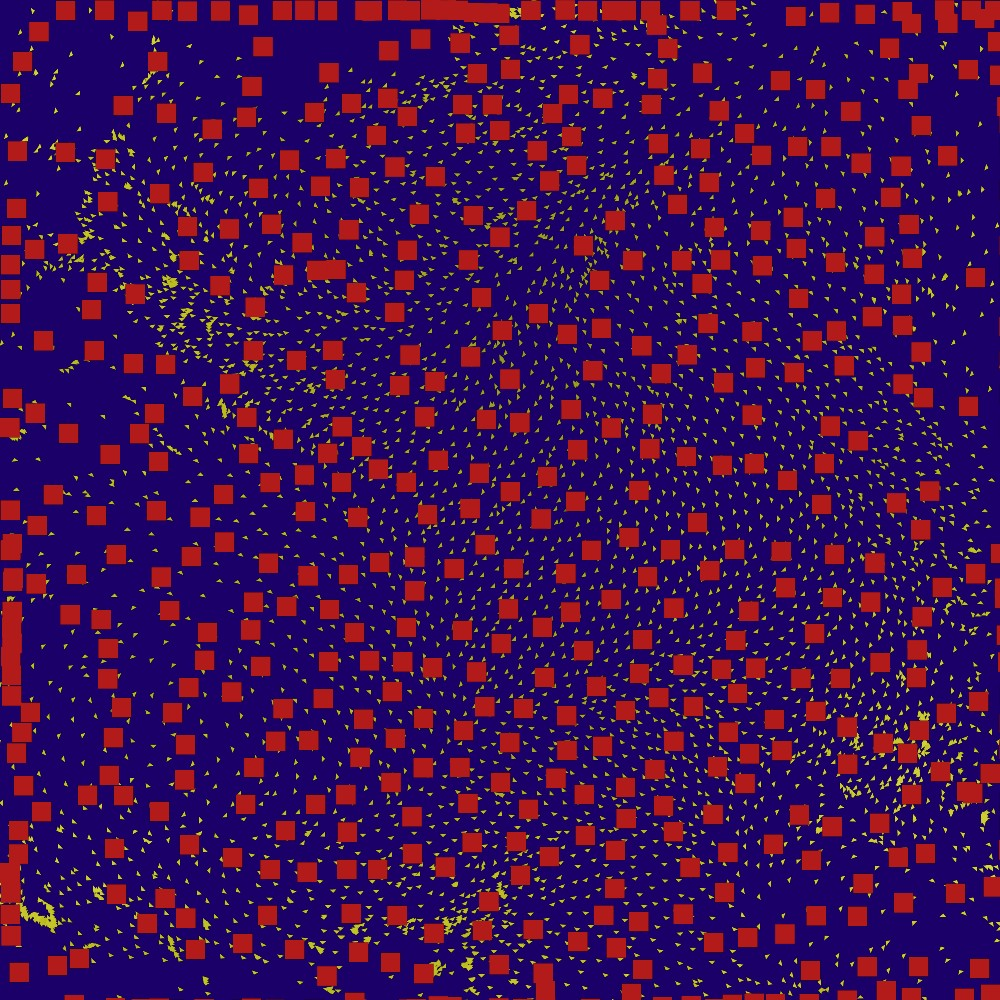
\includegraphics[width=0.95\linewidth]{"img/swarm_2x.jpg"}
			\caption[2 Schwärme]{\textbf{2 Schwärme}}  
		\end{subfigure}		
		\begin{subfigure}{0.5\linewidth}
	 		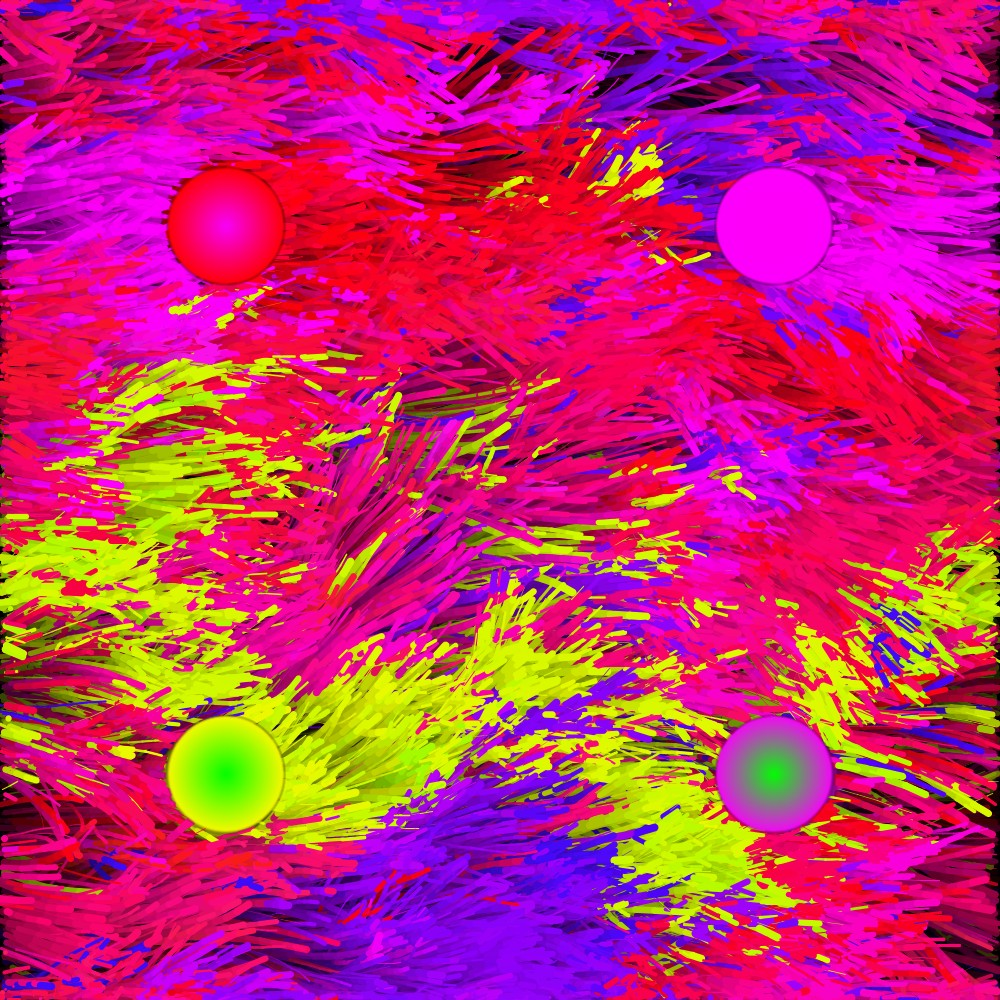
\includegraphics[width=0.95\linewidth]{"img/swarm_fading.jpg"}
			\caption[Colorexplosion]{\textbf{Colorexplosion}}  
		\end{subfigure}	
	\caption[BWinzen:Beispiele Schwarm]{BWinzen:Beispiele Schwarm}
\end{figure}

\subsubsection{BWinzen::LSystem \& BWinzen::LSystemBuilder - Berechnung und Darstellung eines L-System}
	Lindenmayer, ein Biologe aus der Mitte des 20. Jahrhundert, versuchte natürliche Strukturen wie Pflanzen und Bäume mathematisch zu beschreiben. Diese bei seinen Untersuchungen definierten mathematischen Gebilde nennt man heute `Lindenmayer-' bzw. `L-Systemen'.  
	
	Am Anfang eines L-Systems steht ein Alphabet im mathematischen Sinne. Ein Alphabet bezeichnet eine Menge von Zeichen. In einem L-System ist jedem Zeichen eine Visualisierungsregel zugeordnet.\\
	Das Axiom stellt die Startsequenz dar. Es ist eine Tupel beliebiger Elemente aus dem definierten Alphabets des L-Systems. Durch das Axiom wird das L-System initialisiert.\\
	Als Grammatik des L-Systems wird eine Menge von Ersetzungsregel bezeichnet. Diese definieren, welche Zeichen durch eine Reihe anderer Zeichen aus dem Alphabet ersetzet werden. Basiert jede Ersetzungsregel auf einem einzigen Zeichen, welches durch beliebig viele Zeichen ersetzt werden kann, handelt es sich um ein kontextfreies L-System. Gibt es Regeln, bei denen mehrere zusammenhängende Zeichen ersetzt werden, wird es als kontextsensitives L-System bezeichnet \cite{prusinkiewicz1990algorithmic}. Der im Rahmen dieser Arbeit implementierte Generator erzeugt kontextfreie L-Systeme.\\
	In jedem Iterationsschritt werden die Regeln der Grammatik auf die aktuelle Sequenz der Zeichen angewendet. So verändert sich die Sequenz in jedem Iterationsschritt.\\
	Ein Beispiel:
	\begin{itemize}
	\setlength\itemsep{-0.2em}
	\item[] Alphabet = {A,B,+,-}
	\item[] Axiom = A
	\item[] Regeln:
		\begin{itemize}
		\setlength\itemsep{-0.2em}
			\item[1.]A = AB
			\item[2.]B = +A-
		\end{itemize}
	\end{itemize}
	\begin{itemize}
	\setlength\itemsep{-0.2em}
		\item[] 0.Iteration Axiom = A 
		\item[] 1.Iteration AB \quad \quad \quad \quad \quad \quad \quad \quad \quad \quad \quad \quad \quad //Anwendung von Regel 1 
		\item[] 2.Iteration AB+A- \quad \quad \quad \quad \quad \quad \quad \quad \quad \quad \quad//Anwendung von Regel 1 und 2 
		\item[] 3.Iteration AB+A-+AB- \quad \quad \quad \quad \quad \quad \quad \quad //Anwendung von Regel 1 und 2 
		\item[] 4.Iteration AB+A-+AB-+AB+A--   \quad \quad \quad \quad  //Anwendung von Regel 1 und 2 
		\item[] 5.Iteration AB+A-+AB-+AB+A-+AB---   \quad  //Anwendung von Regel 1 und 2 
	\end{itemize}

	Bei der Visualisierung wird jedem Zeichen im Alphabet eine bestimmte Bedeutung zugetragen. So kann zum Beispiel `A' und `B' für vorwärts, `+' für eine rechts Drehung um 20\textdegree\:sowie `-' für eine Linksdrehung um 20\textdegree\:stehen. Wenn man nun die Zeichenkette und die damit Verbunden Zeichenanwendungen mit einem virtuellen Stift nachzeichnet entsteht ein Bild. \\
	Eine Erweiterung der Möglichkeiten eines L-Systems entsteht durch den Einsatz eines FIFO-Speichers. Ein Beispielhafte Belegung von Zeichen wäre:\\
	 Bei dem Zeichen `$[$' wird die aktuellen Position gesichert bei der zugehörigen `$]$' Klammer wird die aktuelle Position wieder geladen.\\
	 So können beispielsweise Verästelung entstehen. Iterationsbedingte Faktoren die Längen und Winkel ändern, ermöglichen eine große Anzahl an zusätzlich darstellbaren Formen.\\
	 Ersatzregeln können auch bedingt formuliert werden, sodass sie nur unter bestimmten Voraussetzungen angewendet werden. Im Zuge des Praktikums wurde auf diesen letzten Schritt der Erweiterung verzichtet und anstelle dessen die Mehrfachbelegung von Variablen in den Ersetzungsregeln erlaubt. Wenn 2 Regeln auf derselben Variable anwendbar sind, entscheidet der Zufall welche von ihnen Verwendung findet. Das in der Konfiguration auswählbare L-System `geordnetes Chaos' benutzt dieses Prinzip um wahlweise eine Ellipse zu zeichnen oder den Baum weiter fortzusetzen.\\
Die `LSystem' Klasse spiegelt das L-System in einem Iterationsschritt dar. Sie enthält das Alphabet (ein Set aus `AlphabetLetter's), die aktuelle Sequenz, sowie alle Ersetzungsregeln. Mit \textit{LSystem nextIteration()} kann das L-System der nächsten Iteration errechnet und instantiiert werden.\\
Die `LSystemTree' Klasse ist für die Visualisierung des L-Systems zuständig. Die erste rekursive Implementation der Visualisierung resultierte in sehr schlechter Performance. Um diesem Problem entgegenzuwirken wurde die Errechnung der Zeichen von dem eigentlichem Zeichenvorgang abgekoppelt. So kann die Zeichenanweisung in mehreren Threads vorberechnet werden und zudem für den mehrmaligen Gebrauch im Cache gespeichert werden.
 Performance und User-Experience mit dem L-System-Generator konnten durch diese Änderung im Algorithmus massiv verbessert werden. Im Rahmen dieser Anpassung wurde die `LSystemTree' Klasse abstract und eine rekursive sowie eine nicht rekursive Variante für die Benutzung vorbereitet. Beide Varianten brauchen unterschiedliche Visualiserungsregeln bzw. Berechnungsregeln. Aktuell sind fast alle auswählbaren L-Systeme auf die nicht rekursive Variante migriert.\\
	Die Benutzung von Farbgradienten bei der Darstellung ist durch die Umstellung auf einen nicht rekursiven Algorithmus leicht möglich. Jede Linie kennt nun die eigene relative Position zum Ausgangspunkt. Die Darstellung fängt immer im Punkt 0,0 an wird anschließend rotiert und verschoben. So wird die Farbe nach Abstand zum Ausgangspunkt errechnet. Das Beispiel `Sierpinski Dreiecke' verdeutlicht dies.

\paragraph{Beschreibung der Parameter für BWinzen::LSystem:}
	Der L-System Generator kann durch 2 Schnittstellen konfiguriert werden. Diese Unterscheidung wurde gewählt, da der Aufwand ein L-System mit Regeln und Axiom einzugeben sehr hoch ist. Durch diese Implementation kann entweder auf vordefinierte L-Systeme zurückgegriffen oder die Parameter manuell konfiguriert werden. Eine Zusammenfassung in einem einzigen Abschnitt der GUI war aufgrund des generischen Aufbaus des Generator-Konfigurationsbereiches nicht möglich. Die Form einer zweiten Eingabemaske macht ein Konfiguration möglich, ohne auf speziell für diesen Zweck entwickelte GUI-Elemente zurückgreifen zu müssen.\\
	Für den `LSystemBuilder' sind folgende Zeichen des Alphabets schon vorbelegt.\\
	Bei `$[$' wird die aktuellen Position gesichert und bei der zugehörigen `$]$' Klammer wird die aktuelle Position wieder geladen.\\
	\indent + ist eine Rechtsdrehung.\\
	\indent - ist eine Linksdrehung.\\
	\begin{itemize}
	\setlength\itemsep{-0.1em}
		\item\textit{Axiom:} (Nur BWinzen::LSystemBuilder)Definieren eines Axioms
		\item\textit{Rule0-5:} (Nur BWinzen::LSystemBuilder)Definieren der Regeln der Grammatik
		\item\textit{Winkel:} (Nur BWinzen::LSystemBuilder) Winkel für eine Rechtsdreheung bei + und eine Linksdrehung bei - 
		\item\textit{LSystem:} (Nur BWinzen::LSystem)Wählen eines vordefinierten LSystems
		\item\textit{Anzahl:} Die Anzahl der LSysteme die vom Generator dargestellt werden sollen.
		\item\textit{Größe:} Die Größe des LSystems.
		\item\textit{gleiche Größe:} Aktiviert - alle erzeugten Darstellungen haben die gleiche Größe.  Deaktiviert - gewählte Größe stellt einen Maximalwert dar. Die eigentliche Größe wird durch eine (Pseudo)Zufallszahl bestimmt.
		\item\textit{Iterationen:} Anzahl der Iterationen, die dargestellt werden.
		\item\textit{Iterationsverzögerung:} Anzahl an Frames, die für einen Iterationsschritt gewartet wird.
		\item\textit{Strichfarbe:} Die Auswahl dient als Grundlage zur Berechnung der Farbe der Darstellungen. 
		\item\textit{Strichstärke:} Die Strichstärke der Darstellung.
		\item\textit{Farbmodus:} siehe \ref{parametrisierung} Allgemeine Parametrisierung>>Farbmodus
		\item\textit{Alpha Wert:} Setzt den Alpha Wert der Darstellungen. 
		\item\textit{KoopModus Orientierung:}  siehe \ref{parametrisierung} Allgemeine Parametrisierung>>KoopModus Orientierung
		\item\textit{Reihenfolge Umkehren:} Wenn die Option gewählt wurden ist, wird zu erst die höchste Iteration des L-Systems gezeichnet und danach die niedrigeren Iterationen. Bei vielen L-Systemen erlangt die Darstellung dadurch eine Art Tiefe wenn zwischen den Iterationen die Farbe variiert. 
		\item\textit{Rotation:} Wenn die Option gewählt wird startet die Darstellung des L-Systems mit einem zufälligen Anfangswinkel.
		\item\textit{XOffset/YOffset:} (Nur BWinzen::LSystemBuilder)Definiert einen X-/Y-Offset, der auf die zufällige Positionierung auf dem Bildschirm addiert wird. So kann das Wachstum der Darstellung Berücksichtigung finden. Ohne den Y-Offset würde eine Darstellung von Bäumen dazu führen das der unter Teil des Bildschirmes sehr leer wirkt. Da nur die dünnen Anfangs-`Stämme' gezeichnet werden.
	\end{itemize}
\paragraph{Beispiele:}
	Folgende Beispiele können im Konfigurator unter MenuBar>>Beispiel>>BWinzen>>LSystem ausgewählt werden.
		\subparagraph{a)Einfaches L-System:} Einfache Darstellung eines L-Systems in der 4.Iteration.\\
	\indent\indent Axiom = F\\
	\indent\indent Winkel = 30 \\
	\indent\indent Regeln: \\
	\indent\indent\indent 1. F = FF+[+F-F-F]-[-F+F+F] \\
	\indent\indent Zusatzregeln:\\
	\indent\indent\indent Die Länge der repräsentierenden Linie zu F wird in jeder Iteration halbiert.
	
	\subparagraph{b)Sierpinski Dreieck:} Dargestellt sind Sierpinski Dreiecke in der 6.Iteration. Die Farben sind zufällig und der Gebrauch von Farbgradient ist sichtbar.\\
	\indent\indent Axiom = F+G+G\\
	\indent\indent Winkel = 120 \\
	\indent\indent Regeln: \\
	\indent\indent\indent 1. G = GG \\
	\indent\indent\indent 2. F = F+G-F-G+F 
	\subparagraph{c)Milkyway:} Dargestellt sind Stern ähnliche L-Systeme in verschiedenen Größen, wie zum Beispiel Koch-Schneeflocken.
	\subparagraph{d)AutumnBlues:} Verschiedene Baum ähnliche L-Systeme in Herbstfarben.
	 
	
\begin{figure}[H]
	\begin{subfigure}{0.5\linewidth}
		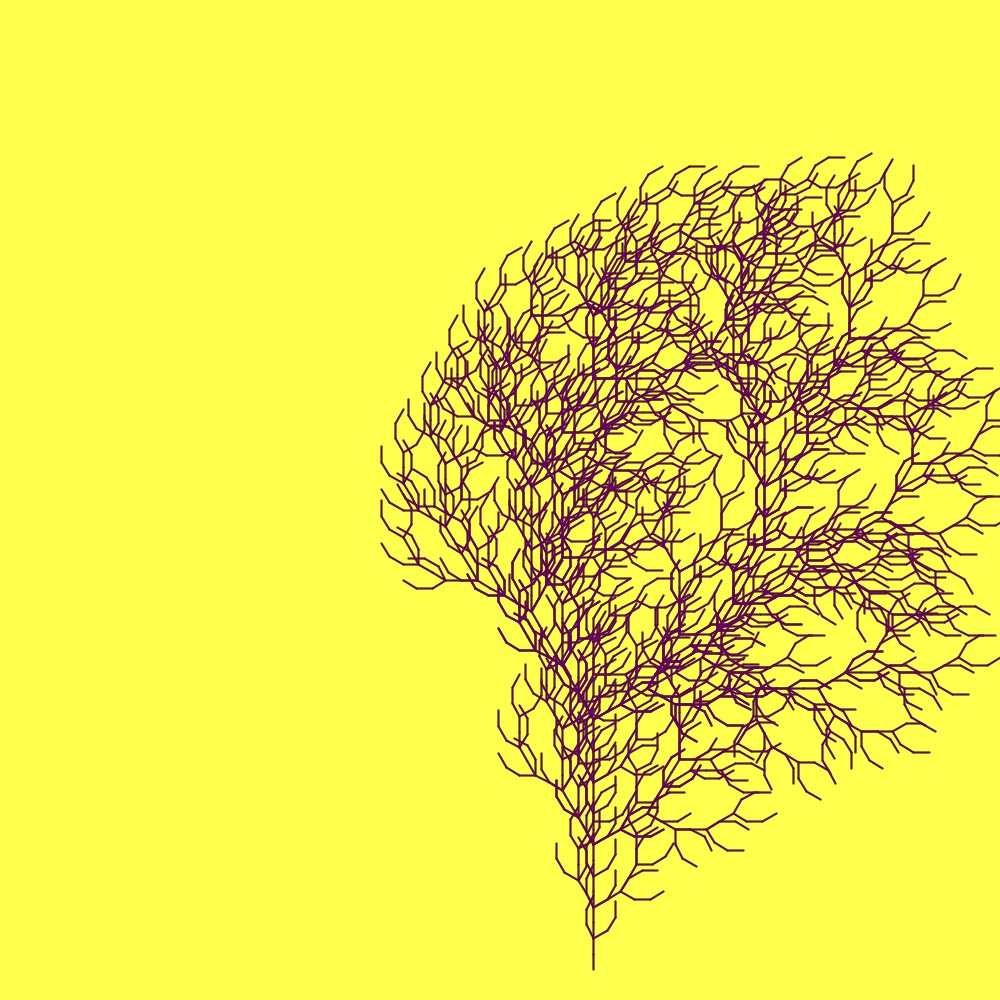
\includegraphics[width=0.95\linewidth]{"img/lsystem_simple.jpg"}
		\caption[Einfaches L-System]{\textbf{Einfaches L-System}}  
	\end{subfigure}
	\begin{subfigure}{0.5\linewidth}
		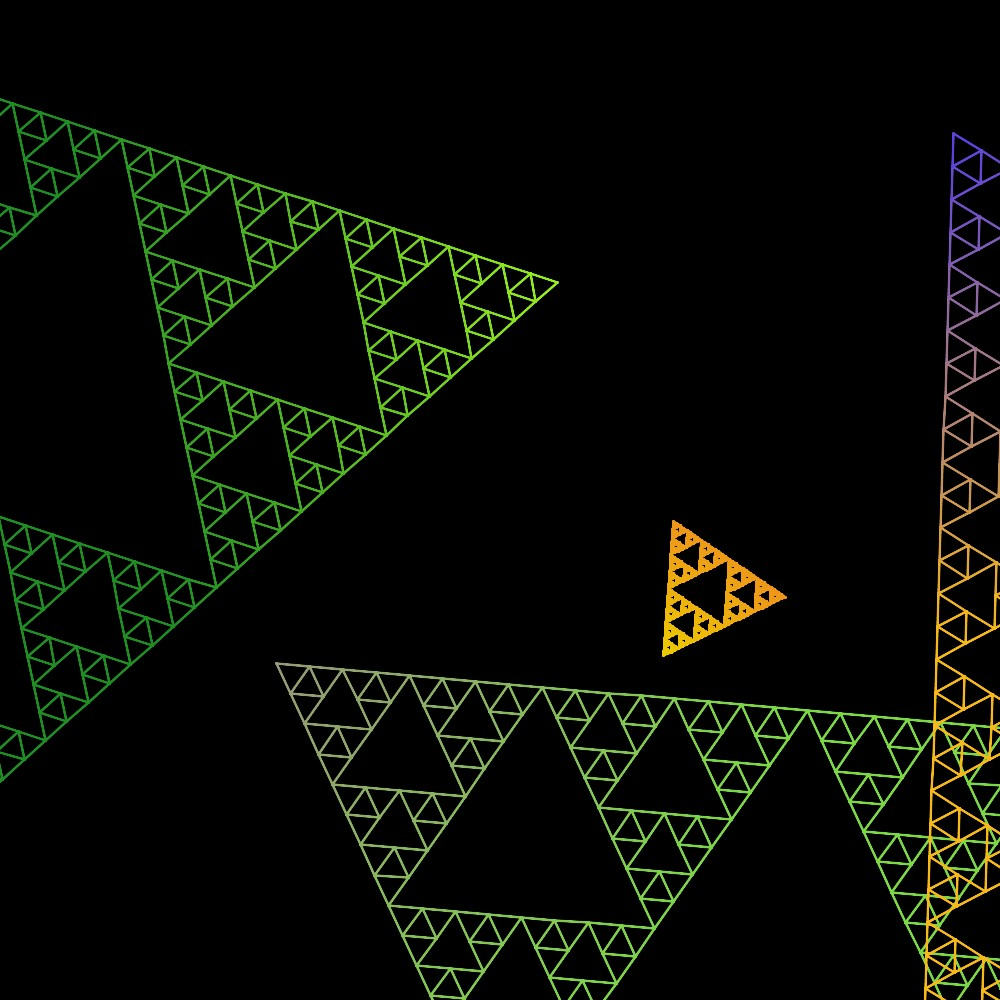
\includegraphics[width=0.95\linewidth]{"img/lsystem_sierpinski.jpg"}
		\caption[Sierpinski Dreieck]{\textbf{Sierpinski Dreieck}}  
	\end{subfigure}		
	\begin{subfigure}{0.5\linewidth}
 		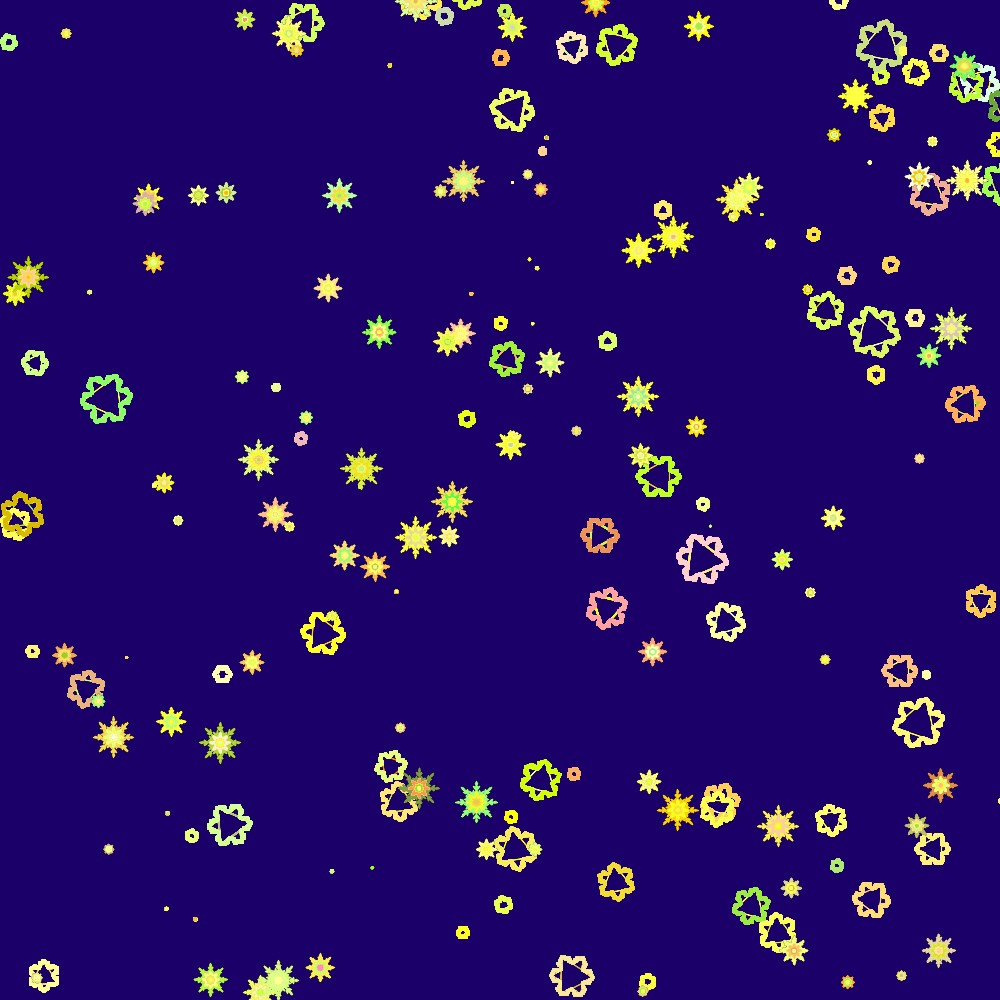
\includegraphics[width=0.95\linewidth]{"img/lsystem_milkyway.jpg"}
		\caption[Milkyway]{\textbf{Milkyway}}  
	\end{subfigure}	
	\begin{subfigure}{0.5\linewidth}
 		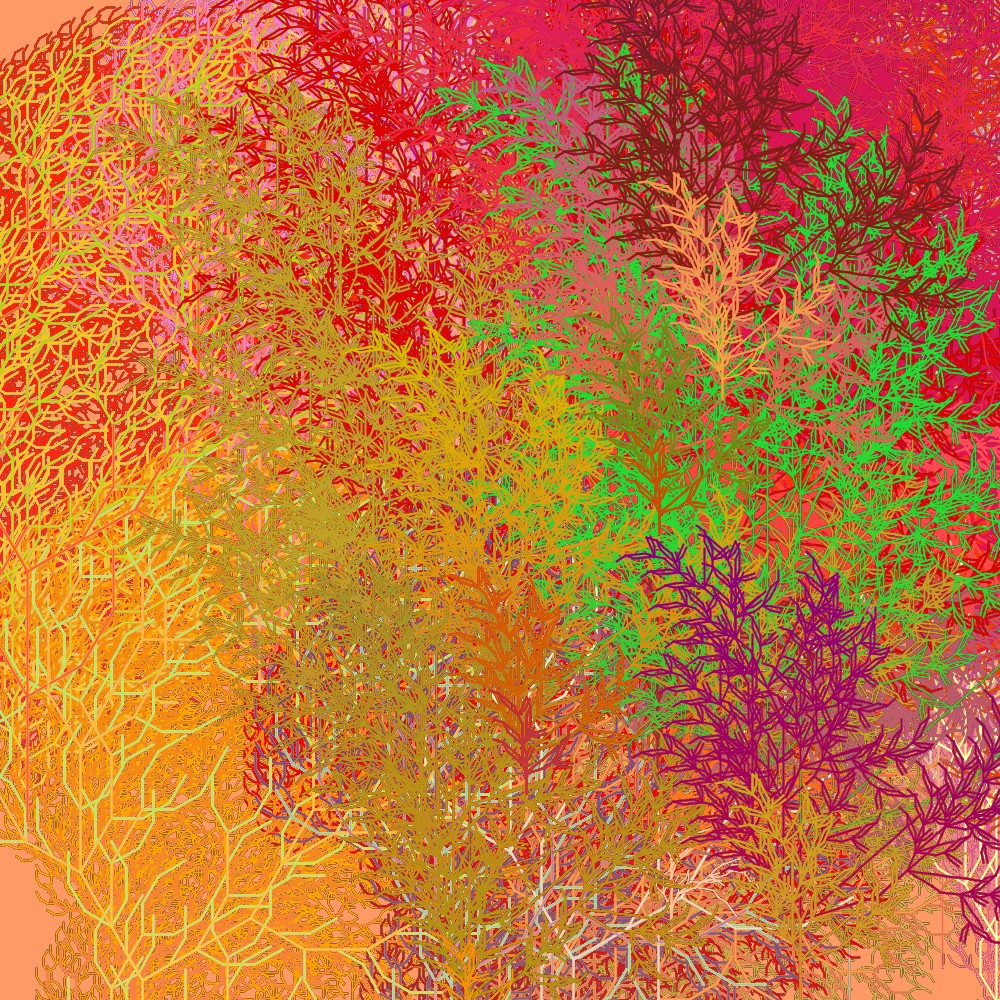
\includegraphics[width=0.95\linewidth]{"img/lsystem_autumn.jpg"}
		\caption[AutumnBlues]{\textbf{AutumnBlues}}  
	\end{subfigure}	
	\caption[BWinzen:Beispiele L-System]{Beispiele L-System}
\end{figure}

	
\subsubsection{BWinzen::3DImageEvolution - Evolutionsprinzipien}
		Im Jahr 1859 veröffentlichte Charles Darwin sein Buch ``On the Origin of Species''. Dieses stellt aus heutiger Sicht einen der größten Meilensteine der Biologie dar. Das Prinzip ``Survival of the fittest'' umschreibt die Tatsache, dass die Entwicklung von Lebewesen nicht gezielt abspielt. Vielmehr werden Individuen aussortiert, welche nicht an die natürlichen Umgebungsfaktoren angepasst sind. Nur wer an die Gegebenheiten angepasst ist, kann bestehen und sich fortpflanzen. Da die Nachkommen ihren Vorfahren physiologisch ähnlich sind haben diese wiederum eine bessere Chance zu überleben und bestimmte Eigenschaften bilden sich so in der Gesamtpopulation heraus. Dieses Prinzip ist heute als Evolutionsprinzip bekannt und hat seinen Weg in viele andere wissenschaftliche Disziplinen gefunden, insbesondere auch in die Informatik. \\
		Heutige Computersysteme rechnen sehr schnell und viele Dinge der Wirklichkeit können durch Modelle mit all ihren Eigenschaften abgebildet werden. So können in wenig Zeit viele Varianten einer Thematik simuliert werden. Dies kann als Basis für einen evolutionäre Entwicklung eines Computermodells genutzt werden.\\
		Bei nicht deterministischen Problemen, kann das Prinzip der Evolution ein passender Ansatz sein um zu einer guten Lösung zu kommen. Wie geeignet die aktuelle Variante des Computermodells in einer Simulation ist, wird durch eine Fitnessfunktion bestimmt. Der Wert der Fitnessfunktion bestimmt die Güte der Simulation und stellt das Gegenstück zur Überlebens- / Fortpflanzungswahrscheinlichkeit in der klassischen Evolution dar.
		 Liefert die Fitnessfunktion einen guten Wert wird die Simulation leicht abgewandelt und überprüft ob noch bessere Werte erreicht werden können. Ist der Wert der Fitnessfunktion schlecht wird der aktuelle Evolutionszweig verworfen.
		
		Der Generator BWinzen::3DImageEvolution besteht aus einem sogenannten Shooter und einer virtuellen Leinwand. Die Leinwand ist auf der Z-Achse versetzt, im Raum platziert. Während der Animation schießt der Shooter Objekte in die Richtung der Leinwand. Eine zweidimensionale Perlin-Noise Funktion hilft dabei die Bewegungen des Shooters flüssig aber zufällig aussehen zu lassen. 
		Wenn die verschossenen Objekte die Leinwand treffen gibt es 2 Möglichkeiten. Wird die Fitness des getroffenen Pixels auf der Leinwand nicht verbessert fliegt das Objekt durch sie hindurch. Wird jedoch die Fitness des getroffenen Pixels verbessert bleibt das Objekt auf der Leinwand haften. Je nachdem wie gut der neue Fitnesswert ist, werden Referenzen (je besser desto mehr) auf den aktuellen Schusses in eine priorisierte Queue abgelegt. Die Queue ist von der Größe begrenzt und hält nur Referenzen mit den besten Fitnesswerten. Die Referenzen enthalten die Farben der verschossenen Objekte als auch die Zielkoordinate.\\
		Zu jedem Zeitpunkt können maximal eine eingestellte Anzahl an Elementen in der Animation umherfliegen. Verlässt ein Element den sichtbaren Bereich bzw. ist zu weit auf der Z Achse fortgeschritten, wird es vom Shooter erneut verschossen.	Die Referenzen in der Queue dienen dabei als bevorzugte Ziele. Solange Referenzen vorhanden sind werden Ziel und Farbe aus der Queue entnommen und leicht verändert. Ist die Queue leer wird die Farbe und Ausrichtung zufällig gewählt.\\
		Als Grundlage für die Fitnessfunktion dient ein Bild, das in der Konfiguration vorgegeben wird. In den Parametern kann für die Fitness-Funktion eine Farbwerteigenschaften als Referenz definiert werden, welche zum Abgleich der aktuellen und der Zielwerte auf den Pixeln genutzt wird.
		
	\paragraph{weitere Schritte:}
		 Aktuell wird die Fitnessfunktion nur auf Farbattribute und zudem nur auf einen einzigen Pixel angewandt. Trifft ein großes Rechteck auf die virtuelle Leinwand, wird nur der Pixel im Zentrum des Rechteckes auf seine Fitness überprüft. Die Fitnessfunktion kann künftig ausgeweitet werden, sodass der gesamte Bereich, den das Element auf der Leinwand abdeckt zur Fitnessfunktion hinzugezogen wird. Zudem ist die Entwicklung anderer Fitnessfunktionen vorstellbar, die nicht nur auf den Farbwert achten, sondern zum Beispiel auf Kanten oder andere Bildeigenschaften.
		 
	\paragraph{Parameter Beschreibung für BWinzen::3DImageEvolution:}
	\begin{itemize}
	\setlength\itemsep{-0.1em}
		\item\textit{Bild:} Auswahl eines Bildes und Grundlage für die Fitnessfunktion
		\item\textit{Max. Anzahl:} Anzahl an gleichzeitig fliegenden Elementen in der Simulation
		\item\textit{Fitness Funktion:} Farbattribute Wert zur Berechnung der Fitnessfunktion 
		\item\textit{Farbe:} dient als Grundlage zur Berechnung der Element Farbe 
		\item\textit{Farbmodus:} siehe \ref{parametrisierung} Allgemeine Parametrisierung>>Farbmodus
		\item\textit{Form:}  siehe \ref{parametrisierung} Allgemeine Parametrisierung>>Form
		\item\textit{Größe:} Die Größe der verschossenen Elemente
		\item\textit{Feste Größe:} Wenn angewählt haben alle Elemente die gewählte Größe ansonsten ist die Größe zufällig und nur durch die Größe als maximal Wert begrenzt.
		\item\textit{KoopModus Start:} Wenn nicht Kooperation via Seed gewählt ist, benutzt der Shooter zur Berechnung seiner Position den Punkt im Kooperationskontext. Dabei wird dieser je nach Auswahl gemieden oder seine nähe gesucht.
		\item\textit{KoopModus Ziel:} Die Elemente vermeiden oder werden vom Punkt im Kooperationskontext angezogen.
		\item\textit{Elem. Geschwindigkeit:} Die Geschwindigkeit, mit der die Elemente fliegen.
		\item\textit{Shooter Geschwindigkeit:} Die Geschwindigkeit, mit der der Shooter sich bewegt / die Perlinois Iterationsschritt Größe.
		\item\textit{Shooter Evolution:} Wenn angewählt Funktioniert die Evolution wie oben beschrieben. Wenn nicht angewählt, wird nur das Bild auf der Leinwand verbessert. Die `Fortpflanzung' von Treffern ist ausgeschaltet.
	\end{itemize}
	\paragraph{Beispiele:}
	Folgende Beispiele können im Konfigurator unter Beispiele>>BWinzen>>3DImageEvolution ausgewählt werden.
		\subparagraph{a)Portrait:} Um das Prinzip deutlicher zu machen, wurde der Shooter, mit Hilfe der Kooperation, in die linke obere Ecke platziert. So verdeckt er nicht das entstehende Bild.\\
			Die gewählte Fitnessfunktion beachtet den errechneten Grauwert einer Farbe. Man kann in der Abbildung deutlich die Auswirkungen der Evolution sehen. Zum einen gibt es gezielte Partikelstrahlen mit ähnlichen Farbwerten und auf dem Bild sind immer wieder Bereiche erkennbar, die auf den gleichen Evolutionären Ursprung zurück gehen. So sind in der Kinnpartie gelbe neben pinken Bereiche. Wenn die Farben in Grauwerten umgerechnet würden, wären sie sehr ähnlich. Die Bereiche sind jedoch initial von einem gelben bzw. pinken Partikel getroffen wurden, der sich fortgepflanzt hat.
	\subparagraph{b)Eule:}Das Bild der Eule wird mit grauen Linien nachgezeichnet. Die Fitnessfunktion basiert auf Grauwerten.
	\subparagraph{c)Papagei:} Das Bild des Papageis wird mit Punkten mit gaußverteilten Zufallsfarben um einen Blauton nachgezeichnet. Die Fitnessfunktion basiert auf den Blauwerten des Bildes. Aus einer farbigen Fotografie im klassischen Sinne entsteht so ein Bild, welches auf die Blauwerte reduziert wird. Alle anderen Farbkanalwerte werden nicht durch die vorgegebene Fitness Funktion beachtet.	
\pagebreak
	\begin{figure}[H]
		\begin{subfigure}{0.5\linewidth}
 		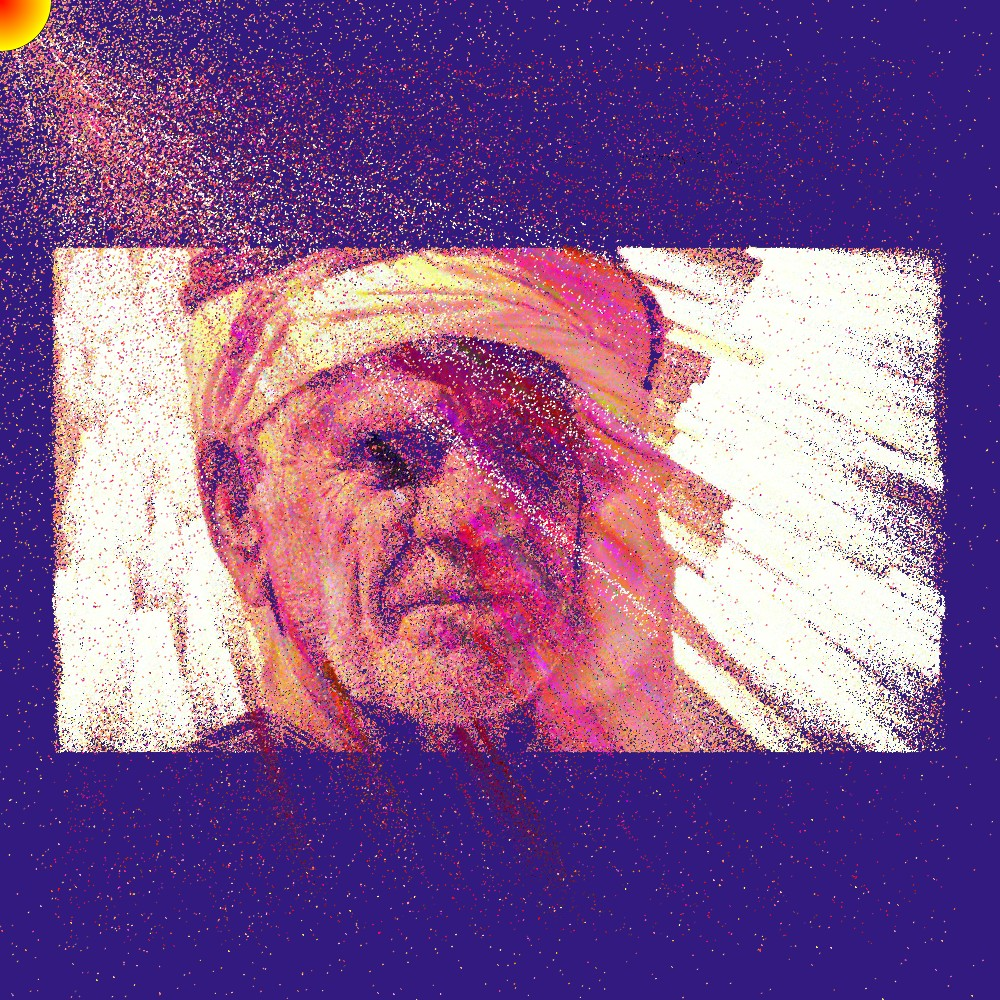
\includegraphics[width=0.95\linewidth]{"img/3dimageevolution_potrait.jpg"}
		\caption[Portrait]{\textbf{Portrait}}  
		 \end{subfigure}
		\begin{subfigure}{0.5\linewidth}
 		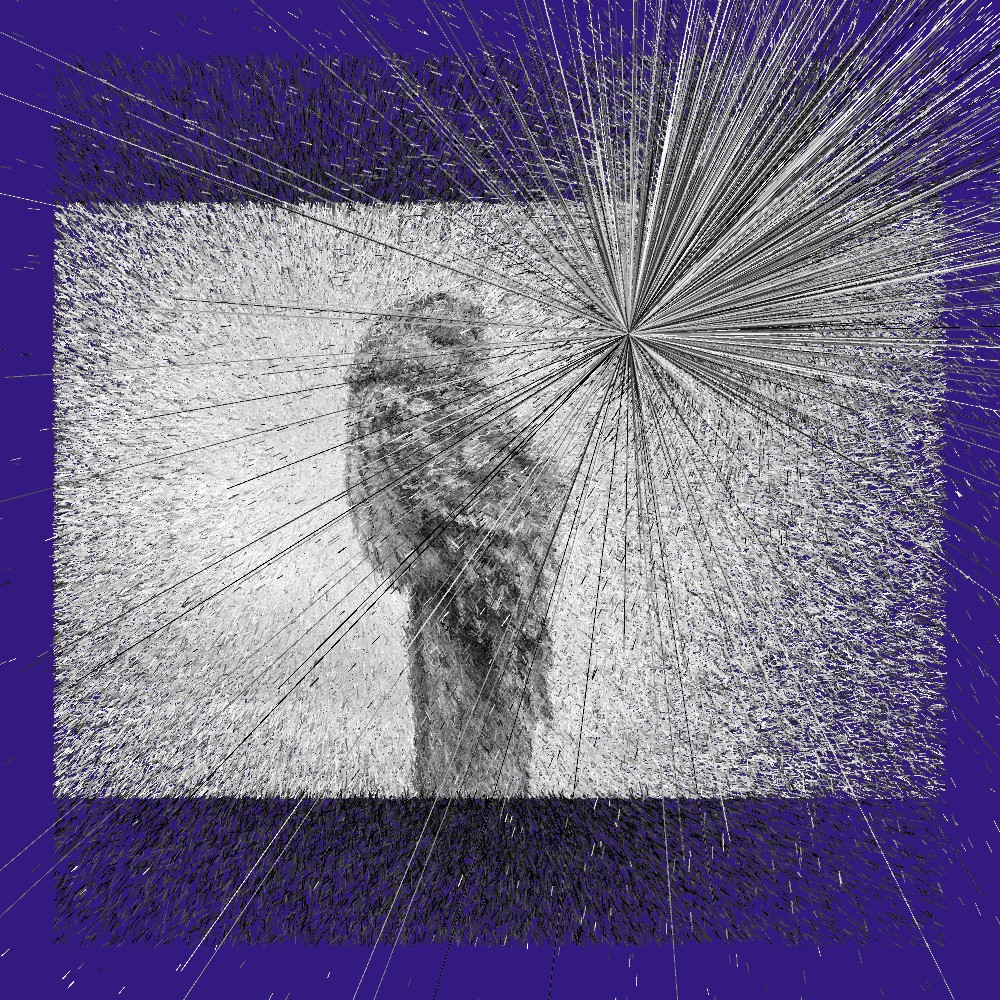
\includegraphics[width=0.95\linewidth]{"img/3dimageevolution_owl.jpg"}
		\caption[Eule]{\textbf{Eule}}  
		 \end{subfigure}
		\begin{subfigure}{0.5\linewidth}
 		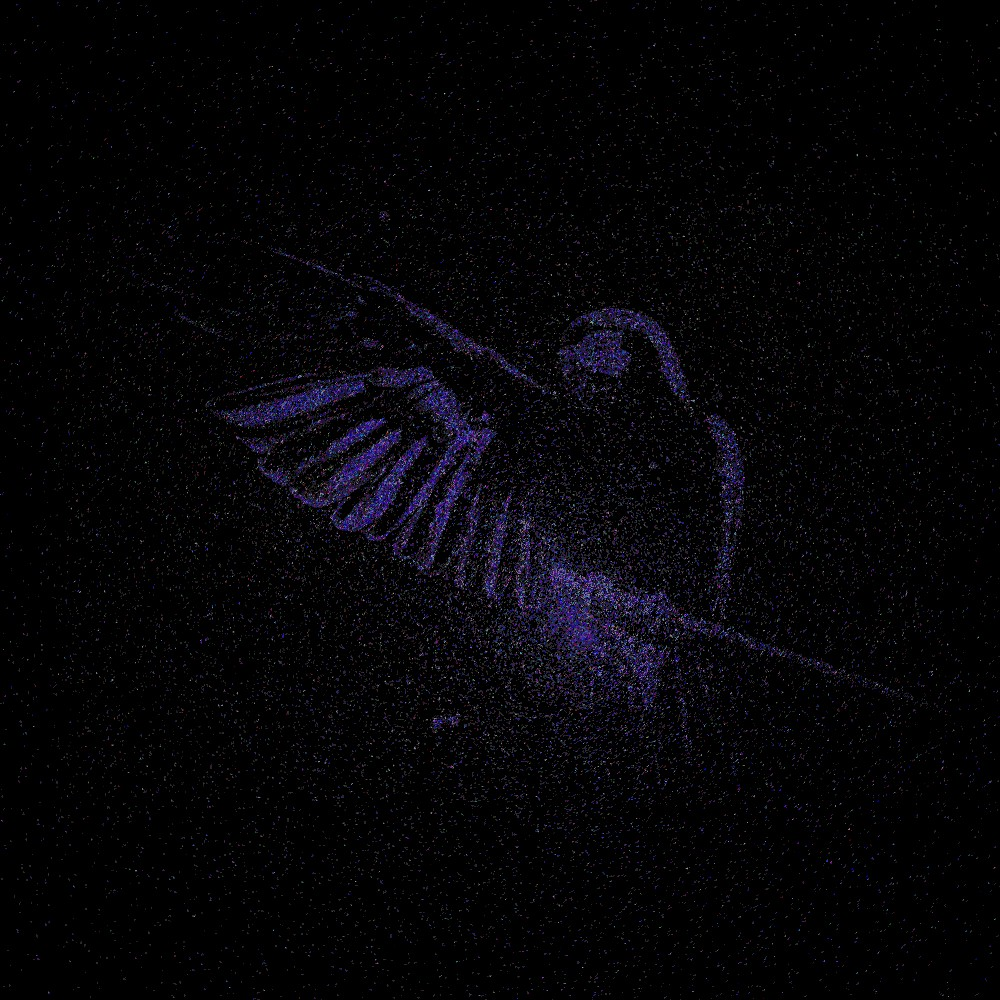
\includegraphics[width=0.95\linewidth]{"img/3dimageevolution_parrot.jpg"}
		\caption[Papagei]{\textbf{Papagei}}
		\end{subfigure} 
		\caption[BWinzen:Beispiele 3DImageEvolution]{Beispiele 3DImageEvolution}
	\end{figure}

\subsubsection{Kooperation}
	Folgende Beispiele können im Konfigurator unter MenuBar>>Beispiele>>BWinzen>>Kooperation ausgewählt werden. Die Algorithmen benutzen alle Arten der beschriebenen Kooperationsmöglichkeiten.
	\begin{figure}[H]
		\begin{subfigure}{0.5\linewidth}
 		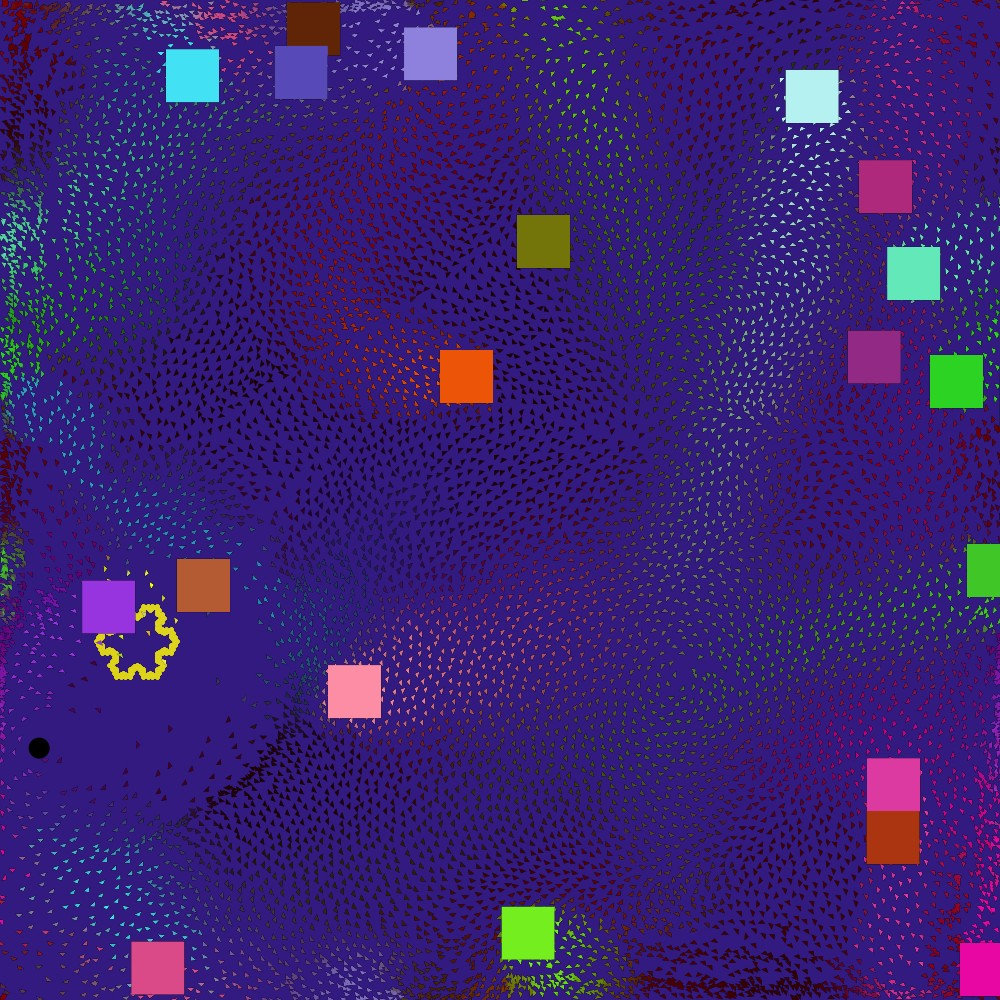
\includegraphics[width=0.95\linewidth]{"img/coop1.jpg"}
		\caption[Jäger \& Gejagte]{\textbf{Jäger \& Gejagte}}  
		 \end{subfigure}
		\begin{subfigure}{0.5\linewidth}
 		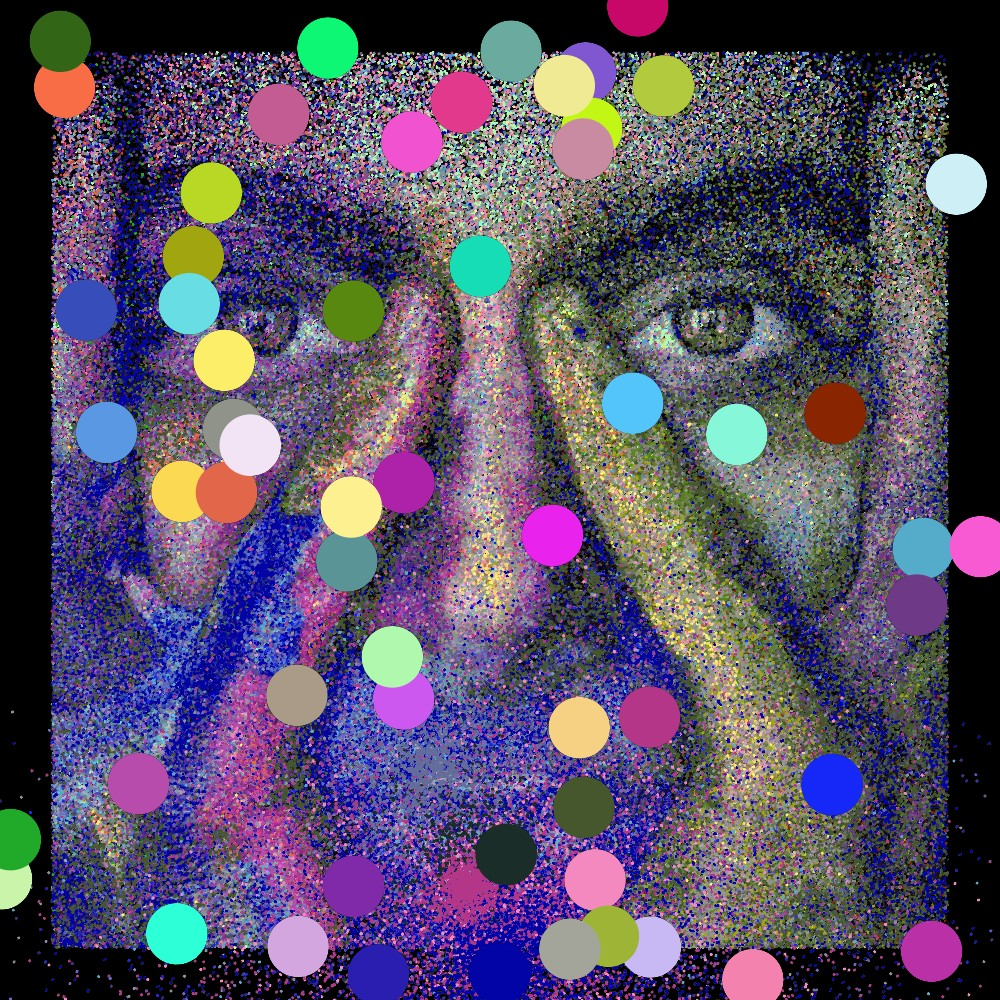
\includegraphics[width=0.95\linewidth]{"img/coop2.jpg"}
		\caption[ImageEvoColorInduction]{\textbf{ImageEvonColorInduction}}  
		 \end{subfigure}
		\begin{subfigure}{0.5\linewidth}
 		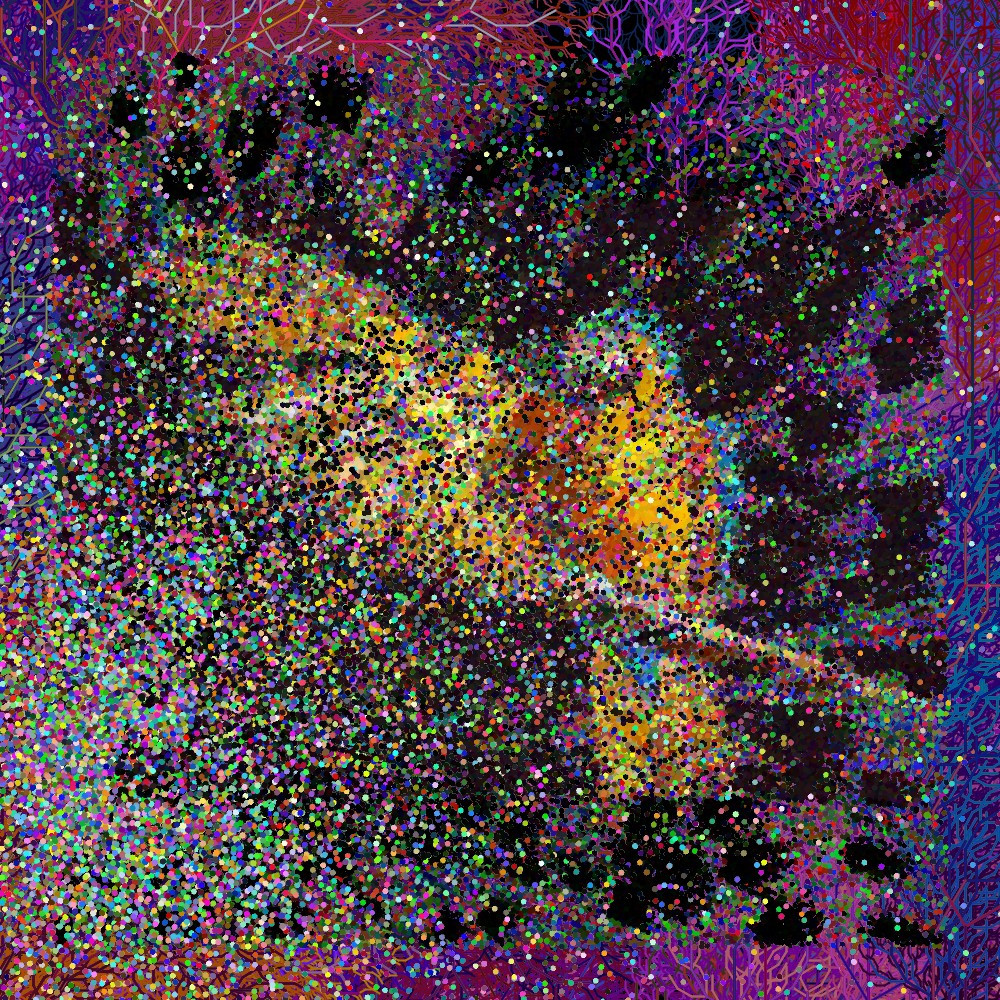
\includegraphics[width=0.95\linewidth]{"img/coop3.jpg"}
		\caption[Regenwald]{\textbf{Regenwald}} 
		\end{subfigure} 
		\caption[BWinzen:Beispiele Kooperation]{Beispiele Kooperation} 
	\end{figure}
\subparagraph{a)Jäger \& Gejagte:} 	Die Komposition besteht aus 4 Generatoren. Bei drei der verwendeten Generatoren handelt es sich um Schwarm Generatoren, der Vierte ist ein L-System. Der erste Schwarm besteht aus großen Quadraten. Sie geben ihre Farbe an die Dreiecke des nächsten Schwarms weiter, wenn ihre Farbe den Anforderungen an die Farbübernahme entspricht - in diesem Fall mindestens ein Farbkanalwert über 0xC4. Zudem versucht der Schwarm aus Dreiecken die Position des schwarzen Kreises im dritten Schwarm zu vermeiden. Der schwarze Kreis wiederum wird vom L-System angezogen.		
\subparagraph{b)ImageEvoColorInduction:} Die Komposition besteht aus einem Schwarm Generator und dem 3DImageEvolution Generator. Der 3DImageEvolution Generator ist so parametrisiert, dass immer der aktuelle Farbwert eines Pixels in der Gesamtkomposition übernommen wird. So dienen die großen Kreise des Schwarms als Farbreservoir für den Shooter. 		 
\subparagraph{c)Regenwald:}	Die Komposition besteht aus einem L-System Generator und einem 3DImageEvolution Generator. Zudem wurden 2 HilfsGeneratoren eingesetzt. Der erste Hilfsgenerator verdrängt das L-System von der Mitte der zweite Hilfsgenerator haftet den Shooter der 3DImageEvolution in die linke untere Ecke. Für den 3DImageEvolution Generator wurde dasselbe Foto verwendet wie im Beispiel `Papagei' verwendet. Allerdings wird in diesem Fall als Referenz für die Fitnessfunktion eine RGB-Skala gewählt.


\subsubsection{Allgemeine Parametrisierung}\label{parametrisierung}
In den unterschiedlichen Generatoren werden Faktoren wie Farbwahl und Form der fliegenden Elemente mehrfach verwendet. Die Logik für dieses Verhalten wurde in Klassen gekapselt und so für die Mehrfachnutzung bereitgestellt.\\
Fliegende Elemente bei denen die Position, sowie die Geschwindigkeit eine Rolle spielen finden sich sowohl in der Schwarm Simulation als auch in der 3DImageEvolution. Die gemeinsamen Eigenschaften konnten in einer Klasse `FlyingObject' untergebracht werden. Um dem `FlyingObject' ein Verhalten zu geben ermöglicht das Enum `Form' den Zugriff auf ein Lambda, das den Zeichenvorgang abstrahiert.
\begin{itemize}
	\setlength\itemsep{-0.1em}
		\item\textit{Farbmodus:} 
			\begin{itemize}
			\setlength\itemsep{-0.1em}
				\item\textit{Einfarbig:}
						Alle Darstellungen haben die gewählte Farbe	
				\item\textit{Gaußverteilte Zufallsfarben um Auswahl:}
						Die Grundlage zur Errechnung der Zufallsfarbe erfolgt über die gewählte Farbe.
						Jeder Channel wird mit folgender Funktion bestimmt \\
						$(int) Math.max(0, Math.min(255, colorChannel + 50 * randomGaussian));$\\
						.randomGaussian ist eine gaußverteilte Zufallszahl zwischen -1 und 1 und wird für jeden R, G und B-Wert neu berechnet.
				\item[]\textbf{Für folgende Farbmodi ist die gewählte Farbe irrelevant}
				\item\textit{Zufällige Farben:} Darstellungen haben zufällige Farbe 
				\item\textit{Zufälliges Grau:} Darstellungen haben zufälligen Grauwert 		
				\item\textit{Aktuelle Pixelfarbe übernehmen:} Die aktuelle Farbe des Pixels in dem die Darstellung startet wird übernommen. 	
			\end{itemize}
	\item\textit{Form:} Folgende Formen können aktuell gewählt werden {Kreise, Linien, Pole, Rechtecke, Quadrate, Dreiecke, Zufällige Formen}
	\item\textit{KoopModus Orientierung:}  siehe \ref{parametrisierung} Allgemeine Parametrisierung>>KoopModus Orientierung
			\begin{itemize}
			\setlength\itemsep{-0.1em}
				\item\textit{Kooperation via Seed:} Die Kooperation findet nur über den Seed zur Zufallsvariablenbestimmung statt. 
				\item\textit{Kooperation via Abstoßung:} Die Darstellung vermeiden den Punkt im Kooperationskontext, sowohl der Anfangswachstum als auch die Richtung des Wachstums wird beeinflusst.
				\item\textit{Kooperation via Anziehung:} Die Darstellungen suchen die Nähe des Punkt im Kooperationskontext.
			\end{itemize}
\end{itemize}

%\bibliographystyle{babplain}
%\bibliography{../mciLiteratur}
\end{document}